\documentclass[main.tex]{subfiles}

\begin{document}

  \section{Computational aspects}

   \subsection{Complexity analysis}

   We recall the parameters of the problem: we consider a superelliptic curve $\cu$ given by
   $\caff:y^m=f(x)$ with $f \in \C[x]$ separable of degree $n$. The genus $g$ of $\cu$ satisfies
   $$g \leq \frac{(m-1)(n-1)}2=O(mn).$$

   Let $D$ be some desired accuracy (a number of digits). The computation of
   the Abel-Jacobi map on $\cu$ has been decomposed into the
   following list of tasks:
   \begin{enumerate}
       \item computing the $(n-1)$ vectors of elementary integrals,
       \item computing the big period matrix $\Omega=(\OA,\OB)$ \eqref{m-eq:OAOB},
       \item computing the small period matrix $\tau = \OA^{-1}\OB$ \eqref{m-eq:tau},
       \item evaluating the Abel-Jacobi map at a point $P \in \cu$,
   \end{enumerate}
   all of these to absolute precision $D$.

   Let $N(D)$ be the number of points of numerical integration.
   If $m=2$, we have
   $N(D)=O(D)$ using Gauss-Chebychev integration, while $N(D)=O(D\log D)$
   via double exponential integration.

   For multiprecision numbers, we consider that the multiplication has
   complexity $M(D)=O(D \log^{1+\varepsilon}D)$,
   while simple transcendental functions (log, exp, sinh,\dots) can be evaluated
   in complexity $T(D)=O(D\log^{2+\varepsilon} D$).
    Moreover, we assume that inversion and multiplication of a $g \times g$ matrix can be done using
    $O(g^{\eta})$ multiplications for some constant $2 < \eta < 3$.
   
   \subsubsection{Computation of elementary integrals}

   For each elementary cycle $\gamma_e\in \Gamma$, we evaluate numerically the vector of $g$
   elementary integrals from \eqref{m-eq:periods} as sums of the form
   \begin{equation}
       \int_{-1}^1\frac{\varphi_{i,j}(u)}{(1-u^2)^{\frac jm}}\du
           \approx \sum_{k=1}^N w_k\frac{x_k^{i-1}}{y_k^j}
   \end{equation}
   where $N$ is the number of integration points, $w_k,u_k$ are integration weights and points,
   $x_k=u_k+\frac{b+a}{b-a}$ and $y_k=\ytab(u_k)$.

   We proceed as follows:
   \begin{itemize}
   \item for each $k$, we evaluate the absissa and weight $u_k,w_k$ using
       a few \footnote{this can be reduced to evaluating only one exponential
       and a few multiplications} trigonometric or hyperbolic functions,
   \item we compute $y_k=\ytab(u_k)$ using $n-2$ multiplications and one $m$-th root,
       as shown in \S \ref{m-subsec:computing_roots} below;
   \item starting from $w_k\frac{1}{y_k}$, we evaluate all $g$ terms $w_k\frac{x_k^{i-1}}{y_k^j}$
       each time either multiplying by $x_k$ or by $\frac{1}{y_k}$, and add each to the corresponding
       integral.
   \end{itemize}

   Altogether, the computation of one vector of elementary integrals takes
   \begin{equation}\label{eq:elem_int_complexity}
    E(D) := N(D)T(D)+N(D)(n-1)M(D)+N(D)gM(D)
   \end{equation}
    operations,
   so that depending on the integration scheme we obtain:
   \begin{thm}\label{thm:complexity_integrals}
       Each of the $(n-1)$ elementary vector integrals can be computed to precision $D$ using
       \begin{itemize}
           \item $O(D^2\log^{1+\varepsilon} D (g + \log^{1+\varepsilon} D))$ operations, if $m=2$,
           \item $O(D^2\log^{1+\varepsilon} D (g + \log^{2+\varepsilon} D))$ operations, if $m>2$.
       \end{itemize}
   \end{thm}
   \begin{proof}
     Plugging in $N(D),T(D),M(D)$ in equation \eqref{m-eq:elem_int_complexity} and using that $n-1 = O(g)$.
   \end{proof}


   \subsubsection{Big period matrix}

   One of the nice aspects of the method is that we never compute
   the dense matrix $\OC\in\C^{g\times 2g}$ from \eqref{m-eq:OC}, but
   keep the decomposition of periods in terms of the elementary integrals
   $\int_{\gamma_e}\omega_{i,j}$ in $\C^{g\times (n-1)}$.

   Using the symplectic base change matrix $S$ introduced
   in \S~\ref{m-subsec:symp_basis}, the homology basis is given
   by equations of the form
   \begin{equation}
       \label{eq:base_change_cycles}
       \alpha_i = \sum_{e,l} s_{e,l}\gamma_e^{(l)}
   \end{equation}
   where $\gamma_e,e\in E$ spans the elementary cycles
   and $l\in\Z/m\Z$ their shifts,
   and $s_{e,l}\in\Z$ are coefficients of the matrix $S$. 

   We use \eqref{m-eq:periods} to compute the coefficients of the big period
   matrix $(\OA,\OB)$, so that each term of \eqref{m-eq:base_change_cycles}
   involves only a fixed number of multiplications.

   In practice, these sums are very sparse and their coefficients are very small integers
   (less than $m$), so that the change of basis is performed using $O(gD\log D)$ operations.

   However we have no proof of this fact, so that we state the far from optimal
   result
   \begin{thm}
       Given the $(n-1)\times g$ elementary integrals to precision $D$,
       we compute the big period matrix using $O(g^2D\log D)$ operations.
   \end{thm}

   \subsubsection{Small period matrix}

   Finally, the small period matrix is obtained as $\tau=\OA^{-1}\OB$,
   i.e. one $g\times g$ matrix inversion and one multiplication, which can be done using
   $O(g^{\eta})$ multiplications.

   
   \subsubsection{Abel-Jacobi map}
   
  This part of the complexity analysis is based on the results of Section \ref{m-sec:comp_ajm} and assumes that we already computed a big period matrix and all related data.
   
  Let $E(D)$ be the number of operations needed to compute a vector of $g$ elemenatary integrals  (see \eqref{m-eq:elem_int_complexity}). The complexity class of $E(D)$ in $O$-notation is given in
  Theorem \ref{m-thm:complexity_integrals}.
  
   \begin{thm} \
   \begin{itemize}
     \item[(i)] For each finite point $P \in \caff$ we can compute $\int_{P_0}^P \bar\w$ to precision $D$ using 
      $E(D)$ operations. 
     \item[(ii)] For each infinite point $P_{\infty} \in \cu$ we can compute $\int_{P_0}^{P_{\infty}} \bar\w$ to precision $D$ using
      \begin{itemize}
       \item[$\bullet$] a few vector additions in $\C^g$, if $\delta = \gcd(m,n) = 1$,
       \item[$\bullet$] $n E(D)$ operations in the case of Theorem \ref{m-thm:ajm_inf_ord1},
       \item[$\bullet$] $n(\nu+M)E(D)$ operations  in the case of Theorem \ref{m-thm:ajm_inf_ordgt1}.
      \end{itemize}
      \item[(iii)] Reducing a vector $v \in \C^g$ modulo $\Lambda$ can be done using $O(g^{\eta})$ multiplications.
    \end{itemize}
  \end{thm}
   \begin{proof}
    \begin{itemize}
     \item[(i)] Follows from combining the results from \S \ref{m-subsec:ajm_ram_pts} and Remark \ref{m-rmk:ajm_finite_int}.
     \item[(ii)] The statements follow immediately from \S \ref{m-subsec:ajm_inf_cop}, Theorem \ref{m-thm:ajm_inf_ord1} and Theorem \ref{m-thm:ajm_inf_ordgt1}.
     \item[(iii)] By \S \ref{m-subsec:lat_red}, the reduction modulo the period lattice requires one $2g \times 2g$ matrix inversion and one multiplication.
    \end{itemize}
   \end{proof}
   

   \subsection{Integration parameters}

   \subsubsection{Double-exponential case}

   We use the parametrization
   $\partial Z_r = \set{ z = \tanh(λ\sinh(t+ir), t\in\R }$.

   The distance from a point $p$ to $Z_r$ can be computed
   applying Newton method to the scalar product function
   $f(t) = \Re(\overline{z'}(p-z))$, where $z = \tanh(λ\sinh(t+ir))$
   and starting point $t=\Re(z^{-1}(p))$.

   Unfortunately the solution may not be unique, so we also use ball arithmetic to compute a rigorous
   bound on the boundary of $Z_r$.

   \paragraph{Choice of $r$}

   We try to minimize the number $N$ of integration
   points obtained from equation
   \eqref{eq:de-parameters} by an appropriate choice
   of parameter $r$.
   
   Writing $u_k = \tanh(λ\sinh(t_k+ir_k))$, we must choose
   $r<r_0=\min_k r_k$ to ensure $u_k\not\in Z_r$.

   For all $k$ such that $r_k > r_0$, we can compute
   explicitely the distance $d_k=\dist(u_k,Z_{r_0})<\dist(u_k,Z_r)$.
   
   For $k$ such that $r_k=r_0$, we write for small $ε>0$
   \[ \dist(u_k,Z_{r-ε}) = ε D_k + O(ε^2) \]
   where
   \[ D_k = \abs{\frac{\partial u_k}{\partial r_k}} = \abs{\frac{λ \cosh(t_k+ir_k)}{\cosh(λ\sinh(t_k+ir_k))^2}} \]
   
   Let $U_0$ be the set of branch points $u_k$ reaching the minimum
   value $r_0$, and 
   \[ M_0 = (\prod_{u_k\in U_0} D_k\prod_{u_k\not\in U_0}d_k)^{-j/m} \]
   then the integrand is bounded on $Z_{r_0-ε}$ by
   \[ M_2 = M_0 ε^{-\frac{j\#U_0}m} (1+O(ε)) \]
   so that
   \[ h = \frac{2π(r_0-ε)}{A-λ\log(ε)+O(ε)} \]
   for constants $A=D+\log(2B(r_0,α)M_0)$ and $λ=j\#U_0/m$.

   The maximum is obtained for $ε(A+λ-λ\log(ε))=λr_0$,
   we can take
   \[ ε = \frac{λr_0}{A+λ(1+\log\frac{A+λ}{λr})} \]
   
   \subsubsection{Gauss-Chebychev case}

   If we write $r=\cosh(ρ)$, then we have a parametrization
   $ε_r = \set{ \cosh(ρ+it) = \cos(t-iρ), t\in]-π,π] }$
   of the ellipse.

   \begin{figure}[H]
       \begin{center}
       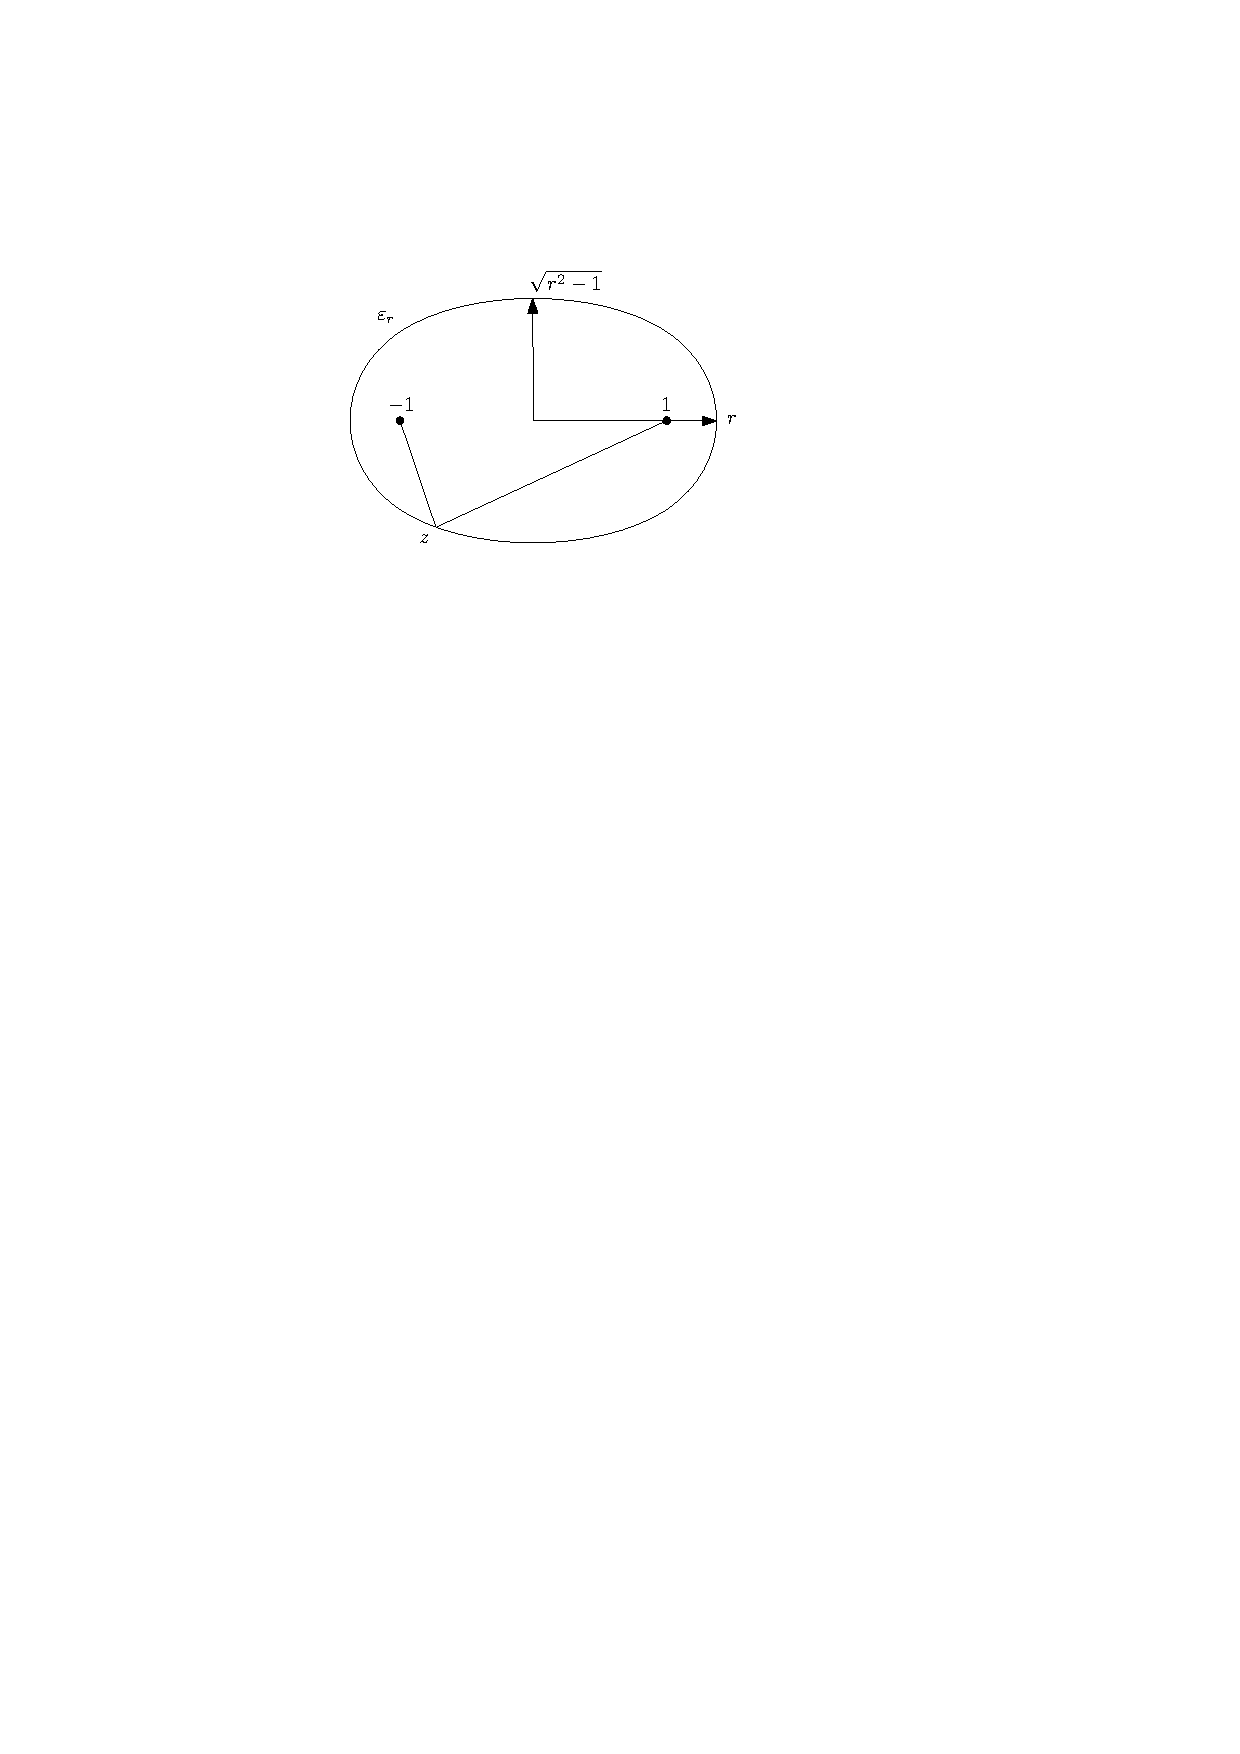
\includegraphics[width=5cm]{images/ellipse.pdf}
   \end{center} \caption{Ellipse parameters.}
   \label{fig:ellipse}
   \end{figure}

   The sum of its semi-axes lengths becomes $r+\sqrt{r^2-1}=e^{ρ}$
   and one needs 
   \[
       n = \frac{D+\log(2πM(r)+e^{-D})}{2ρ}
   \]
   to have $\abs{E(n)}\leq e^{-D}$.

   The distance $d_k=\dist(u_k,ε_r)$ from a branch point $u_k$
   to the ellipse $ε_r$ can be computed
   applying Newton method to the scalar product function
   $f(t) = \Re(\overline{z'}(u_k-z))$, where $z = \cos(t-iρ)$
   and starting point $t=\Re(\arccos(u_k))$. By convexity of the ellipse,
   the solution is unique on the quadrant containing $u_k$.

   \subsubsection{Choice of $r$}
   
   Let $r_k = \frac{\abs{u_k-1}+\abs{u_k+1}}2$. We need to choose
   $r<r_0=\min_k r_k$ (so that $u_k\not\in ε_r$) in order to minimize
   the number of integration points.

   For all $k$ such that $r_k > r_0$, we compute
   explicitely the distance $d_k=\dist(u_k,ε_{r_0})<\dist(u_k,ε_r)$.
   
   For $k$ such that $r_k=r_0$, we use first order approximation
   \[ \dist(u_k,Z_{r-ε}) = ε D_k + O(ε^2) \]
   where
   \[ D_k = \abs{\frac{\partial u_k}{\partial r_k}} = \abs{\sin(t_k-ir_k)} \]
 
   Let $U_0$ be the set of branch points $u_k$ reaching the minimum
   value $r_0$, and 
   \[ M_0 = (\prod_{u_k\in U_0} D_k\prod_{u_k\not\in U_0}d_k)^{-j/m} \]
   then the integrand is bounded on $Z_{r_0-ε}$ by
   \[ M_2 = M_0 ε^{-\frac{j\#U_0}m} (1+O(ε)) \]
   so that
   \[ h = \frac{2π(r_0-ε)}{A-λ\log(ε)+O(ε)} \]
   for constants $A=D+\log(2B(r_0,α)M_0)$ and $λ=j\#U_0/m$.

   The maximum is obtained for $ε(A+λ-λ\log(ε))=λr_0$,
   we can take
   \[ ε = \frac{λr_0}{A+λ(1+\log\frac{A+λ}{λr})} \]
   
   \subsection{Implementation tricks}

   Here we simply give some further ideas used in our implementation to improve constants.

   \subsubsection{Improving branch points}

   As we saw in Section \ref{m-sec:numerical_integration}, the number of integration points
   closely depends on the configuration of branch points.

   In practice the tau constant of double-exponential integration is usually bigger than $0.5$
   for random points, but we can exhibit bad configurations with $τ\approx 0.1$. In this case
   however, we can perform a change of coordinate by a Moebius transform
   $x\mapsto \frac{ax+b}{cx+d}$ to redistribute the points more evenly.

   Improving $τ$ from $.1$ to say $.6$ immediately saves a factor $6$ on the running time.

  \subsubsection{Computing products of complex roots}\label{subsec:computing_roots}

  For numerical integration of the integrals in \eqref{m-eq:periods}
  we need to evaluate
  \begin{equation*}
   \ytab(u) = \prod_{u_k\in U^-} \sqrt[m]{u-u_k}\prod_{u_k\in U^+}\sqrt[m]{u_k-u}
  \end{equation*}
  for $u \in [-1,1]$. Instead of computing $(n-2)$ $m$-th roots for each
  integration point, we compute $q \in \frac12\Z$ such that
  \begin{equation*}
   \ytab(u) = \zeta^q \Big( \prod_{u_k\in U^-}(u-u_k) \prod_{u_k\in U^+} (u_k-u) \Big)\mr
  \end{equation*}
 which can be done by tracking
  the winding number of the product while staying away from the branch cut
  of the $m$-th root.
  For complex numbers $z_1,z_2 \in \C$ we can make a diagram of
  $\frac{\sqrt[m]{z_1}\sqrt[m]{z_2}}{\sqrt[m]{z_1z_2}} \in \{ 1, \zeta,
  \zeta^{-1} \}$, depending on the position of $z_1,z_2$ and their product
  $z_1z_2$ in the complex plane, resulting in the following Lemma:

  \begin{lemma}\label{lemma:wind_numb}
  Let $z_1,z_2 \in \C  \setminus  ]\infty,0]$. Then,
  $$\frac{\sqrt[m]{z_1}\sqrt[m]{z_2}}{\sqrt[m]{z_1z_2}} = \begin{cases}
                                                           \zeta, \quad \text{if} \quad \Im(z_1), \Im(z_2) > 0 \quad \text{and} \quad \Im(z_1z_2) < 0 , \\
                                                           \zeta^{-1}, \text{if} \quad \Im(z_1), \Im(z_2) < 0 \quad \text{and} \quad \Im(z_1z_2) > 0 , \\
                                                           1, \quad \text{otherwise}.
                                                         \end{cases}$$
   For $z \in ]\infty,0]$ we use $\sqrt[m]{z} = \zeta^{\frac{1}{2}} \cdot \sqrt[m]{-z}$.
  \end{lemma}
  \begin{proof}
   Follows from the choices for $\sqrt[m]{\cdot}$ and $\zeta$ that were made in \S \ref{m-subsec:roots_branches}.
  \end{proof}
   This Lemma can easily be turned into an algorithm that computes $q$.

   \subsubsection{Doing real multiplications}\label{subsec:real_mult}

   During integration, the main complexity comes from the multiplication by numerator
   $x_k=u_k-\frac{b+a}2$, which is usually done $g-m-1$ times for each of
   the $N$ integration points.

   More precisely, as we saw in the proof of Proposition \ref{m-prop:holom_diff}, for each power $j$
   we use the powers $0\leq i\leq n_i = \floor{\frac{nj-δ}m}$, with $\sum n_i = g$.

   However, $x_k$ is a complex number while $u_k$ is real, so it is better to compute
   the integrals with $u_k$ only and make a simple shift on the integral values of the form
   \begin{equation}
       %\left(
       \int_{-1}^1 (u+c)^iF_j(u) \du
       %\right_{0\leq i\leq d_i}
       =
       %\left(
       \sum_{l=0}^i {i \choose l} c^{i-l} \int_{-1}^{1} u^lF_j(u)\du
       %\right_{0\leq i\leq d_i}
   \end{equation}

   This saves a factor almost $2$ on the running time.

\biblio
\end{document}
